% vim: set textwidth=78 autoindent:

\section{Plugins di QGIS}\label{sec:plugins}\index{plugin}

% when the revision of a section has been finalized, 
% comment out the following line:
%\updatedisclaimer

Quantum GIS è stato progettato con un'architettura estensibile tramite plugin. Ciò permette di aggiungere nuove caratteristiche e funzioni
all'applicazione. Molte delle caratteristiche in QGIS sono in effetti implementate come plugin di
base \textbf{Core} o \textbf{Esterni} contribuiti dagli utenti.\index{plugin!tipi} 

\begin{itemize}
\item \textbf{Plugins Core} sono mantenuti dal team di sviluppo di QGIS e fanno automaticamente parte di ogni distribuzione QGIS.
Sono scritti in uno dei due seguenti linguaggi: C++ o Python.
Ulteriori informazioni riguardanti i plugin core sono disponibili nella sezione  \ref{sec:core_plugins}.
\item \textbf{Plugin Esterni} sono attualmente tutti scritti in Python.
Sono immagazzinati in archivi dei pacchetti esterni e mantenuti dai singoli autori.
Possono essere aggiunti a QGIS usando il plugin core chiamato \filename{Plugin Installer}.
Ulteriori informazioni riguardanti i plugin esterni sono disponibili nella sezione \ref{sec:external_plugins}.
\end{itemize}

\subsection{Gestione dei plugin}\label{sec:managing_plugins}
\index{plugin!gestione} 

La gestione dei plugin consiste nella loro abilitazione o disabilitazione usando il plugin \filename{Plugin Manager}.
I plugin esterni devono prima essere installati usando il plugin \filename{Plugin Installer}.

\subsubsection{Abilitare un Plugin Core}\label{sec:load_core_plugin} 

L'abilitazione di un Plugin Core si ottiene dal menu principale \mainmenuopt{Plugins} > \dropmenuopttwo{mActionShowPluginManager}{Manage Plugins...}.\index{plugin!gestione}

\begin{figure}[ht]
   \begin{center}
   \caption{Plugin Manager \nixcaption}\label{fig:pluginmanager}\smallskip
   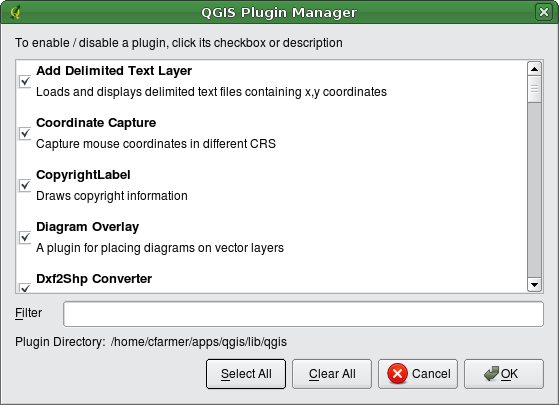
\includegraphics[clip=true, width=14cm]{pluginmanager}
\end{center}
\end{figure}

Il gestore dei plugin (QGIS Plugin Manager) elenca tutti i plugin disponibili e il loro stato (abilitato o disabilitato).
I plugin disponibili comprendono sia tutti i Core sia tutti gli Esterni che sono stati aggiunti usando il plugin \filename{Plugin Installer} (vedere la sezione \ref{sec:external_plugins}).
la figura \ref{fig:pluginmanager} mostra la finestra di dialogo del gestore dei plugin QGIS Plugin Manager.
I plugin abilitati vengono "memorizzati" quando si esce dall'applicazione, in maniera tale che al riavvio di QGIS l'utente li trovi già disponibili.

\begin{Tip}\caption{\textsc{Blocco plugin}}\index{blocco}\qgistip{Se vi accorgete che QGIS si blocca all'avvio, la colpa potrebbe essere di un plugin. È possibile disabilitare il caricamento di tutti i plugin modificando il relativo file delle impostazioni (vedere \ref{subsec:gui_options} per localizzarlo). Una volta individuate le impostazioni dei plugin bisogna impostare il valore di ognuno su "false" in modo da impedirne il caricamento. \nix {Per esempio per disabilitare il plugin Delimited text, la modifica da effettuare sul file \$HOME/.config/QuantumGIS/qgis.conf di Linux dovrebbe apparire così: \usertext {Add Delimited Text Layer=false}.} \normalfont Eseguire l'operazione per tutti i plugin della sezione, avviare successivamente QGIS ed aggiungere i plugin uno alla volta tramite il gestore per determinare quale stia causando il problema.}
\end{Tip}

\subsubsection{Caricamento di un plugin esterno in QGIS}\label{sec:load_external_plugin} 

Per integrare i plugin esterni in QGIS si deve prima caricare il plugin \filename{Plugin Installer} come descritto nella sezione \ref{sec:load_core_plugin}.
Successivamente si possono caricare i plugin esterni Python in due passi: 

\begin{enumerate}
\item Scaricare il plugin esterno dall'archivio dei pacchetti usando  \filename{Plugin Installer} (Sezione \ref{sec:python_plugin_installer}).
Il nuovo plugin esterno verrà aggiunto alla lista dei plugin disponibili nel \filename{Plugin Manager}.
\item Caricare il plugin usando il \filename{Plugin Manager}.
\end{enumerate}

\subsubsection{Uso dell'installatore di Plugin Python}\index{plugin!installazione}\label{sec:python_plugin_installer}
\index{plugin!installatore plugin Python}\index{plugin!aggiornamento}

\begin{figure}[ht]
   \begin{center}
   \caption{Installazione di plugin Esterni Python \nixcaption}
\label{fig:plugininstaller}\smallskip
   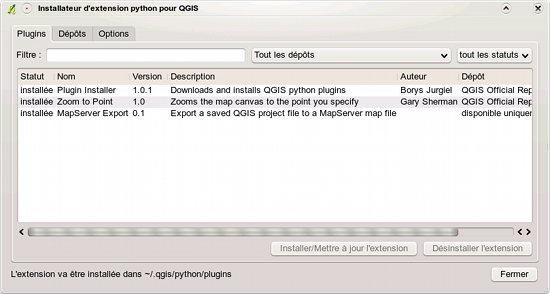
\includegraphics[clip=true, width=14cm]{plugininstaller}
\end{center}
\end{figure}

Per scaricare e installare un plugin python esterno, selezionare il menu \mainmenuopt{Plugins} > \dropmenuopttwo{plugin_installer}{Fetch Python Plugins...}.
Apparirà la finestra \filename{Plugin Installer}  (figure \ref{fig:plugininstaller}) con il tab \tab{Plugins}, contenente la lista sia di tutti i plugin python disponibili negli archivi remoti sia di quelli installati. Ogni plugin può essere:
\begin{itemize}
\item \textbf{not installed} - significa che il plugin è disponibile nell'archivio remoto, ma non ancora installato. Per installarlo, selezionarlo dalla lista e premere il pulsante  \button{Install plugin}.
\item \textbf{new} - idem come sopra, ma il plugin è visto per la prima volta.
\item \textbf{installed} - il plugin è installato. Se è anche disponibile in qualsiasi archivio remoto il pulsante \button{Reinstall plugin} è abilitato. Ma la versione disponibile in remoto è più vecchia di quella installata, appare invece il pulsante \button{Downgrade plugin}.
\item \textbf{upgradeable} - il plugin è installato, ma è disponibile una versione più recente. Il pulsante \button{Upgrade plugin} è abilitato.
\item \textbf{invalid} - il plugin è installato, ma è inutilizzabile. La ragione è spiegata nella descrizione del plugin.
\end{itemize}

\minisec{Plugins tab}

Per installare un plugin, selezionarlo dalla lista e premere il pulsante  \button{Install plugin}. Il plugin è installato nella sua propria directory, per esempio per \nix sotto \filename{\$HOME/.qgis/python/plugins} ed è visibile solo per l'utente che lo ha installato. Vedere una lista di altre subdirectory usate per i plugin specifiche per ogni sistema operativo nella Sezione~\ref{subsec:pyfoursteps}. Se l'installazione va a buon fine, compare un messaggio di conferma. A questo punto andare su \mainmenuopt{Plugins} > \dropmenuopttwo{mActionShowPluginManager}{Manage Plugins...} e caricare il plugin installato.

Se l'installazione fallisce ne viene indicata la ragione. I problemi più frequenti sono correlati a errori di connessione e moduli Python mancanti. Nel primo caso bisognerà attendere alcuni minuti o anche ore, nel secondo è necessario installare nel sistema operativo i moduli mancanti  prima di usare il plugin. \nix{In Linux, i moduli più richiesti dovrebbero essere disponibili nel gestore dei pacchetti}. \win{Per istruzioni sull'installazione in Windows, visitare la homepage del modulo}. Se si usa un proxy, può essere necessario configurarlo nel menu \mainmenuopt{Settings} > \dropmenuopttwo{mActionOptions}{Options} nella scheda \tab{Proxy}.

Il pulsante \button{Uninstall plugin} è abilitato solo se il plugin selezionato è installato e non è un plugin Core. Da notare che se si è installato un aggiornamento (update) di un Core plugin, si può sempre disinstallare tale aggiornamento con il pulsante \button{Uninstall plugin} e ritornare alla versione contenuta nel pacchetto di installazione di Quantum GIS. Ma il plugin non può venir disinstallato.

\minisec{Repositories tab}

La seconda scheda \tab{Repositories} contiene una lista di archivi di plugin disponibili per l'installatore di Plugin. Come impostazione di default viene usato solamente l'archivio ufficiale di QGIS (QGIS Official Repository). Si possono aggiungere archivi contribuiti dagli utenti, incluso l'archivio centrale "QGIS Contributed Repository" ed alcuni altri archivi usando il pulsante \button{Add 3rd party repositories}. Questi archivi contengono un gran numero di plugin più o meno utili, ma bisogna tener presente che non essendo mantenuti dal Team di Sviluppo di QGIS, quest'ultimo non se ne assume la responsabilità.
Si può anche gestire la lista dei plugin manualmente, cioè aggiungere, rimuovere o editare le singole voci. È possibile disabilitare temporaneamente un particolare archivio usando il pulsante \button{Edit...}.

La casella di scelta \checkbox{Check for updates on startup} fa sì che QGIS cerchi gli aggiornamenti e le news dei plugin. Se la funzione è selezionata tutti gli archivi elencati e abilitati nella scheda \tab{Repositories} sono verificati ogni volta che il programma viene aperto. Se è disponibile un nuovo plugin o l'aggiornamento di uno di quelli già installati, compare una messaggio di notifica selezionabile nella Barra di Stato. Se la casella di scelta non è selezionata, la ricerca di nuovi plugin e di aggiornamenti viene effettuata solamente quando si lancia l'installatore di Plugin da menu.

Nel caso di problemi con la connessione internet, può esser visibile durante l'intera sessione di QGIS un indicatore  \textit{Looking for new plugins...} nella Barra di Stato che può causare il blocco del programma alla chiusura. In questo caso deselezionare la casella di scelta.

\subsection{Data Providers}\index{data provider}

I Data Provider sono plugin speciali che danno accesso ad un archivio di dati. Per default, QGIS supporta i layer PostGIS e gli archivi di dati su disco supportati dalla libreria  GDAL/OGR (Appendice \ref{appdx_ogr}).
Un plugin Data Provider estende l'abilità di QGIS di utilizzare altre sorgenti di dati.

I plugin Data Provider sono registrati automaticamente all'avvio di QGIS. Non sono gestiti dal QGIS Plugin Manager, ma usati dietro le quinte quando un tipo di dati viene aggiunto come layer in QGIS.
